\documentclass{standalone}
\usepackage{tikz}
%------------tikz Setup------------

\tikzstyle{ball} = [circle,shading=ball, ball color=black,
    minimum size=1mm,inner sep=1.3pt]
\tikzstyle{miniball} = [circle,shading=ball, ball color=black,
    minimum size=1mm,inner sep=0.5pt]
\tikzstyle{mminiball} = [circle,shading=ball, ball color=black,
    minimum size=0.6mm,inner sep=0.1pt]
\usetikzlibrary{arrows.meta}
\usetikzlibrary{angles, quotes}
\tikzset{>={Latex[length=2mm,width=1.5mm]}}
\tikzset{->-/.style={decoration={markings, mark=at position #1 with
  {\arrow{>}}},postaction={decorate}}}
\usetikzlibrary{decorations.pathmorphing}
\usetikzlibrary{decorations.pathreplacing}
\usetikzlibrary{arrows.meta,calc}
\usetikzlibrary{bending}
\usetikzlibrary{decorations.markings,shapes.geometric}
\tikzset{->-/.style={decoration={markings, mark=at position #1 with
  {\arrow{>}}},postaction={decorate}}}
\tikzset{-|-/.style={decoration={markings, mark=at position #1 with
  {\arrow{stealth}}},postaction={decorate}}}
\tikzset{movearrow/.style 2 args ={
        decoration={markings,
    mark= at position {#1} with {\arrow{#2}} ,
        },
        postaction={decorate}
    }
}


\begin{document}
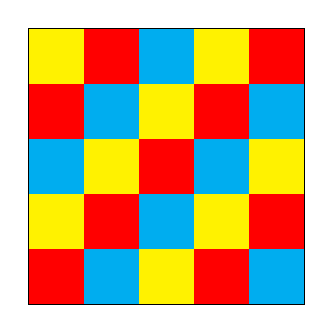
\begin{tikzpicture}[scale=0.7]
    \draw[thick] (0,0) rectangle (5,5);
    \fill[red] (0,0) rectangle (1,1);
    \fill[red] (1,1) rectangle (2,2);
    \fill[red] (2,2) rectangle (3,3);
    \fill[red] (3,3) rectangle (4,4);
    \fill[red] (4,4) rectangle (5,5);
    \fill[red] (3,0) rectangle (4,1);
    \fill[red] (4,1) rectangle (5,2);
    \fill[red] (0,3) rectangle (1,4);
    \fill[red] (1,4) rectangle (2,5);
    \fill[cyan] (1,0) rectangle (2,1);
    \fill[cyan] (2,1) rectangle (3,2);
    \fill[cyan] (3,2) rectangle (4,3);
    \fill[cyan] (4,3) rectangle (5,4);
    \fill[cyan] (0,2) rectangle (1,3);
    \fill[cyan] (1,3) rectangle (2,4);
    \fill[cyan] (2,4) rectangle (3,5);
    \fill[cyan] (4,0) rectangle (5,1);
    \fill[yellow] (0,1) rectangle (1,2);
    \fill[yellow] (1,2) rectangle (2,3);
    \fill[yellow] (2,3) rectangle (3,4);
    \fill[yellow] (3,4) rectangle (4,5);
    \fill[yellow] (2,0) rectangle (3,1);
    \fill[yellow] (3,1) rectangle (4,2);
    \fill[yellow] (4,2) rectangle (5,3);
    \fill[yellow] (0,4) rectangle (1,5);
\end{tikzpicture}
\end{document}